
\documentclass{bredelebeamer}
  \usepackage{booktabs} 
  \usepackage{multirow}
\usepackage{array}
\usepackage[]{color}
\usepackage{blkarray}
\usepackage{tikz}
\usepackage{verbatim}
\usepackage{amsmath,graphicx,centernot}
\usepackage{lipsum}
\usetikzlibrary{arrows,shapes}
\usetikzlibrary{arrows.meta}
\usepackage{subcaption}
\captionsetup{compatibility=false}
\usetikzlibrary{shapes,backgrounds,arrows,automata,snakes,shadows,positioning, mindmap}
\usepackage{amsmath,amssymb,amsthm,mathrsfs,amsfonts,dsfont} 
\usepackage{color, colortbl}
\newcommand\independent{\protect\mathpalette{\protect\independenT}{\perp}}
\renewcommand{\newblock}{}
\def\independenT#1#2{\mathrel{\rlap{$#1#2$}\mkern2mu{#1#2}}}
\tikzset{
  level/.style   = { ultra thick, blue },
  connect/.style = { dashed, red },
  notice/.style  = { draw, rectangle callout, callout relative pointer={#1} },
  label/.style   = { text width=2cm }
  rect/.style = {rectangle, rounded corners, draw=black,
                           minimum width=4cm, minimum height=1cm,
                           text centered, font=\sffamily}
  connect/.style = { dashed, blue }
}


\newcommand{\backupbegin}{
   \newcounter{framenumberappendix}
   \setcounter{framenumberappendix}{\value{framenumber}}
}
\newcommand{\backupend}{
   \addtocounter{framenumberappendix}{-\value{framenumber}}
   \addtocounter{framenumber}{\value{framenumberappendix}} 
}
\DeclareMathOperator*{\argmax}{arg\,max}
%%%%%%%%%%%%%%%%%%%%%%%%%%%%%%%%%%%%%%%%%%%%%%%%



\title[Séminaire Rochebrune]{Inférence de réseaux à partir de mélanges d'arbres}
\subtitle{Encadré par  S. Robin$^{\inst{1}}$ et C. Ambroise$^{\inst{1}\inst{2}$ }}

\institute[]
{
  \inst{1}%
  UMR AgroParisTech / INRA MIA-Paris \\
  \inst{2}%
  LaMME, Evry
  }



\author{Raphaëlle Momal-Leisenring}
% La commande \inst{...} Permet d'afficher l' affiliation de l'intervenant.
% Si il y a plusieurs intervenants: Marcel Dupont\inst{1}, Roger Durand\inst{2}
% Il suffit alors d'ajouter un autre institut sur le modèle ci-dessous.




\date{\today}
% Optionnel. La date, généralement celle du jour de la conférence

\subject{Séminaire Rochebrune}
% C'est utilisé dans les métadonnes du PDF




%%%%%%%%%%%%%%%%%%%%%%%%%%%%%%%%%%%%%%%%%%%%%%%%%%%%%%%%%%%%%%%%%%%%%

\begin{document}
\begin{frame}
  \titlepage
\end{frame}
\section{Introduction}
\begin{frame}{Réseau}
    \begin{itemize}
     \item Réseau : représentation graphique de la structure de dépendance conditionnelle d'un jeu de données.
      \item Inférer un réseau : inférer les arêtes du graph, \textit{i.e.} la structure de dépendance.
    \end{itemize}

    \vspace{1cm}
\begin{columns}
 \begin{column}{0.35\linewidth}
 \begin{flushright}
  \begin{tikzpicture}
     

      %% UN graphe 
      \tikzstyle{every edge}=[-,>=stealth',shorten >=1pt,auto,thin,draw]
      \tikzstyle{every node}=[fill=yellow!40!orange]
      \tikzstyle{every state}=[draw=none,text=black,scale=0.5,
      transform shape,circular drop shadow] 
      
      \node[fill=white] at (2.25,-0.5) ;

      % premier cluster
      \node[state] (A1) at (1.,0) {A};
      \node[state] (A2) at (2.4,0) {B};
      \node[state] (A3) at (1.7,1.5) {C};
      \node[state] (A4) at (1.7,0.7) {Z};
      
        \path (A2) edge [] (A4)
        (A1) edge [] (A4)
        (A3) edge [] (A4);
      

\end{tikzpicture}\\
\end{flushright}
\end{column}
\begin{column}{0.1\linewidth}
\begin{center}
 $\Rightarrow$
\end{center}
\end{column}

\begin{column}{0.55\linewidth}
\begin{flushleft}
 
 Les variables A, B et C sont inépendantes entre elles conditionnellement à la variable Z.
\end{flushleft}

\end{column}

\end{columns}


\end{frame}



%\begin{frame}{Sommaire}
%  \tableofcontents
%  % possibilité d'ajouter l'option [pausesections]
%\end{frame}




\begin{frame}{Exemple de réseau écologique}
\begin{columns}
\begin{column}{0.45\linewidth}

\cite{jakuch}:\\


\begin{itemize}
\item But : identifier les liens de dépendance entre le champignon \textit{E. alphitoïde} présent sur les feuilles du chêne, et les autres micro-organismes présents.\vspace{0.4cm}
\item Utile à la compréhension et au contrôle des maladies chez le chêne.
\end{itemize}

\vspace{0.4cm}
%Variable continue, structure de dépendance modélisée par des copules %gaussiennes utilisant les résidus de Pearson, puis inférence bayésienne du %réseau.
\end{column}
\begin{column}{0.55\linewidth}
\begin{figure}
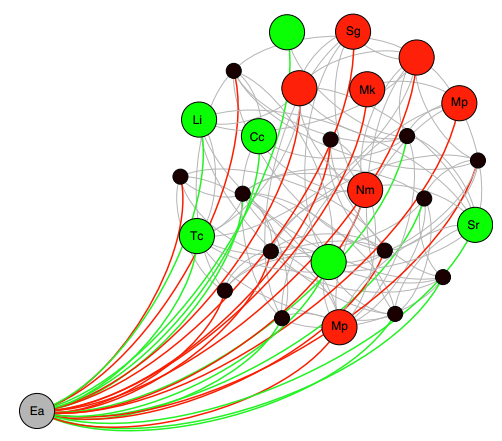
\includegraphics[scale=0.45]{illu_reseau}
\caption{Model of the pathobiome \textit{Erysiphe alphitoides} on oak leaves, source : Jakuschkin \textit{et al.} }
\end{figure}
\end{column}
\end{columns}

\end{frame}

\begin{frame}{Modèle graphique }
\begin{itemize}
\item Clique $C$ d'un graphe $G$: sous-ensemble de noeuds de $G$ qui sont tous liés entre eux.\\

\item Clique maximale $C_{G}$ : aucune autre clique de $G$ ne la contient strictement.\\

\end{itemize}

\begin{exampleblock}{Propriété modèle graphique \cite{Lau96}}
Soit  $Y = (Y_1,...,Y_q)$ et $p$ sa densité. $p$ se factorise selon le graphe non orienté G si :
\[ p(y) \propto \prod_{C \in C_G} \Phi_C (y^C) \]
Et alors G représente la structure d'indépendance conditionnelle entre les $Y_i$.
\end{exampleblock} 
Exemple : $Y=(Y_1,...,Y_4)$ : \\
\begin{columns}
 \begin{column}{0.35\linewidth}
 \begin{flushright}

 \begin{tikzpicture}
     

      %% UN graphe 
      \tikzstyle{every edge}=[-,>=stealth',shorten >=1pt,auto,thin,draw]
      \tikzstyle{every node}=[fill=yellow!40!orange]
      \tikzstyle{every state}=[draw=none,text=black,scale=0.5,
      transform shape,circular drop shadow] 
      
      \node[fill=white] at (2.25,-0.5) ;

      % premier cluster
      \node[state] (A1) at (1.,0) {$Y_1$};
      \node[state] (A2) at (2.8,0.7) {$Y_2$};
      \node[state] (A3) at (1.7,1.5) {$Y_3$};
      \node[state] (A4) at (2,0.7) {$Y_4$};
      
        \path (A2) edge [] (A4)
        (A1) edge [] (A4)
        (A3) edge [] (A4)
        (A3) edge [] (A1);
      

\end{tikzpicture}\\
\end{flushright}
 \end{column}
 \begin{column}{0.6\linewidth}
 \begin{flushleft}
    $p(Y) = \phi_1(Y_1,Y_4) \times \phi_2(Y_2,Y_3,Y_4)$
 \end{flushleft}
 \end{column}
\end{columns}
\end{frame}

\begin{frame}{Cas gaussien (GGM, \textit{Gaussian Graphical Models})}
Soit $Y$ une variable gaussienne multivariée de dimension $d$:

\vspace{0.5cm}
\begin{center}
  $Y=(Y_1,...,Y_d) \sim \mathcal{N}_d(0,\Sigma)$,\\
$\Omega = \Sigma^{-1} = (w_{ij})_{1 \leq i,j \leq d}$. \\
\end{center}


 \vspace{0.5cm}
 L'écriture de la gaussienne permet directement d'obtenir une factorisation :
 \vspace{0.5cm}
\begin{align*}
p(y) &\propto exp(-y^T \Omega y /2)\\
&\propto \prod_{j,k, \omega_{jk} \neq 0 } exp(-y_j w_{jk} y_k /2)  
\end{align*}
\only<2>{
 \begin{columns} 
 \begin{column}{0.5\linewidth}
 \begin{flushright}
\[\Omega=
\left(
\begin{array}{*{4}{c}}
* & 0 & * & *\\
0 & * & 0 & *\\
* & 0 & * & *\\
* & * & * & *
\end{array}
\right)
\]
 \end{flushright}
 \end{column}
 \begin{column}{0.05\linewidth}
\begin{center}
 $\Rightarrow$
\end{center}
\end{column}
 \begin{column}{0.45\linewidth}
 \begin{flushleft}
\vspace{0.5cm}
 \begin{tikzpicture}
     

      %% UN graphe 
      \tikzstyle{every edge}=[-,>=stealth',shorten >=1pt,auto,thin,draw]
      \tikzstyle{every node}=[fill=yellow!40!orange]
      \tikzstyle{every state}=[draw=none,text=black,scale=0.5,
      transform shape,circular drop shadow] 
      
      \node[fill=white] at (2.25,-0.5) ;

      % premier cluster
      \node[state] (A1) at (1.,0) {$Y_1$};
      \node[state] (A2) at (2.8,0.7) {$Y_2$};
      \node[state] (A3) at (1.7,1.5) {$Y_3$};
      \node[state] (A4) at (2,0.7) {$Y_4$};
      
        \path (A2) edge [] (A4)
        (A1) edge [] (A4)
        (A3) edge [] (A4)
        (A3) edge [] (A1);
      

\end{tikzpicture}\\
\end{flushleft}
 \end{column}

\end{columns}}
\end{frame}

\begin{frame}{Inférence de $\Omega$ : le graphical Lasso}
\begin{itemize}
 \item  Estimation parcimonieuse
 \item La log-vraisemblance de  $Y$ s'écrit :
 \[L(Y,\Omega) \propto \frac{n}{2}\log(det(\Omega))-\frac{n}{2} Y^T\Omega Y\]
\end{itemize}


 \begin{exampleblock}{ Le graphical-Lasso (glasso) :}
  Le graphical-Lasso pénalise la norme $l_1$ de la matrice de précision :
  \[\widehat{\Omega}_\lambda = \arg\min_{\Omega \in \mathcal{S}_d^+}\left\{ L(Y,\Omega)+\lambda \sum_{i\neq j} |w_{ij}| \right\}\]
 \end{exampleblock}
 \begin{itemize}
  \item Choix du $\lambda$...
 \end{itemize}

\end{frame}
\section{EM pour mélange d'arbres}
\begin{frame}{Notation}
    \begin{itemize}
        \item $Y$ : tableau de données, de dimension $n\times d$
        \item $d$ : nombre de variables (ex : espèces)
        \item $n$ : nombre d'observations (échantillons)
    \end{itemize}
\end{frame}
\begin{frame}{Arbre de dépendance}
\begin{itemize}
    \item La structure de dépendance des données s'appuie sur un arbre
    \item Vraisemblance de données continues \cite{ChowLiu}:
     
\begin{align*}
\mathds{P}(Y|T) &=\mathds{P}(Y_1|T)\prod_{j=2}^d \frac{\mathds{P}(Y_j,Y_{a_j}|T)}{\mathds{P}(Y_{a_j}|T)}\\
&=\underbrace{\prod_{j=1}^d \mathds{P}(Y_j|T)}_{\text{$A$}}\prod_{(k,l)\in T} \underbrace{\frac{\mathds{P}(Y_k,Y_l|T)}{\mathds{P}(Y_k|T)\times \mathds{P}(Y_l|T)}}_{\psi_{kl}(Y)}\\
&=A\prod_{k,l \in T}\psi_{kl}(Y)
\end{align*}
\item Cas gaussien centré réduit :
\[\log(\mathds{P}(Y|T))   \propto \sum_{k,l\in T}\underbrace{-\frac{n}{2}\log (1-\hat{\rho}_{kl}^2)}_{\log(\hat{\psi}_{kl})}+\sum_k\underbrace{-\frac{n}{2} \log(\hat{\sigma}_k^2)}_{\log(\hat{A})}\]
\end{itemize}
    
\end{frame}
\begin{frame}{Mélange d'arbres}
En fait un mélange sur les arêtes du graph :
\begin{itemize}
    \item Un poids $\beta_{kl}$ est attribué à chaque arête $(k,l)$ possible du graph.
    \item La probabilité de l'arbre de dépendance des données s'écrit alors
    \[ \mathds{P}(T) = \frac{1}{B}\prod_{k,l\in T} \beta_{kl} \text{ , avec } B = \sum_{T\in\mathcal{T}} \prod_{k,l\in T} \beta_{kl} \]
    \item Les poids sont en général fixés à l'avance
\end{itemize}
\end{frame}
\begin{frame}{L'idée}
\begin{center}
L'arbre réel qui structure la dépendance est caché.\\
\vspace{0.5cm}
    \Huge{$\Downarrow$}
    \vspace{0.5cm}
\end{center}

\boiteorange{Construire un algorithme EM avec pour paramètre la loi de l'arbre, avec mise à jour des poids des arêtes.}
    
\end{frame}
\begin{frame}{Algorithme EM : étape E}
\boiteverte{\[ \log(p_\theta (Y) )= \mathds{E}_\theta \left(\log(p_\theta (Y,Z))|Y \right) \underbrace{- \mathds{E}_\theta \left(\log(p_\theta (Y|Z))|Y \right)}_{\text{\normalsize{$\mathcal{H}(p_\theta (Y|Z))$}}} \]
}
 \[ \mathds{P}(Y,T) = \mathds{P}(T)\times\mathds{P}(Y|T)\]
\begin{align*}
 \log(\mathds{P}(Y,T)) &= \sum_{(k,l)\in E_T} \left[ \log(\beta_{kl}) + \log(\psi_{kl})  \right] -\log(B)+\log(A) \\
 &= \sum_{k,l\in V} \mathds{1}_{\{(k,l) \in E_T\}} (\log(\beta_{kl}) + \log(\psi_{kl}) ) -\log(B) +\log(A)
 \end{align*}
  Espérance conditionnelle :
\[ \mathds{E}_\theta[\log(\mathds{P}(Y,T))|Y] =\sum_{k,l\in V} \emph{$\mathds{P}((k,l) \in E_T|Y)$ }(\log(\beta_{kl}) + \log(\psi_{kl}) ) -\log(B) +\log(A)\]
    
\end{frame}


\begin{frame}{Calcul de la probabilité conditionnelle}
\begin{exampleblock}{Théorème du matrix tree (étendu aux réels, \cite{MixtTrees})}
Pour toute matrice symétrique $W=(a_{kl})_{k,l}$, son Laplacien $Q(W)$ se définit par :
 \[\mathcal{Q}_{uv}(W)=
 \begin{cases}
     -a_{uv} & 1\leq u<v \leq n\\
    \sum_{w=1}^n a_{wv} & 1\leq u=v \leq n.
\end{cases}
\]
Alors pour tout $u$ et $v$:
    \[ |Q^*_{uv}(W)|=\sum_{T\in\mathcal{T}} \prod_{\{k,l\}\in E_T} a_{kl} \]
\end{exampleblock}
\only<2>{\begin{align*}
  \mathds{P}((k,l)\in T | Y)&=\sum_{T\in \mathcal{T} : (k,l)\in T}\mathds{P}( T | Y) = \frac{\sum_{(k,l)\in T} \mathds{P}(T)\mathds{P}(Y|T)}{\sum_{T} \mathds{P}(T)\mathds{P}(Y|T)}\\
 &=\frac{\sum_{(k,l)\in T} \prod_{uv} \beta_{uv}  \psi_{uv}(Y)}{\sum_{T} \prod_{uv} \beta_{uv} \psi_{uv}(Y)}\\
 &=1- \frac{|Q^*_{uv}(B\Psi^{-kl})|}{|Q^*_{uv}(B\Psi)|}
 \end{align*}
 }
\end{frame}





\begin{frame}{Algorithme EM : étape M}
But : optimiser les poids $\beta_{kl}$.\\
\[\argmax_{\beta_{kl}} \left\{\sum_{k,l\in V} \tau_{kl}(\log(\beta_{kl}) + \log(\psi_{kl}) ) -\log(B) - n\times cst\right\}\]
\[ \frac{\partial\mathds{E}_\theta[\log(\mathds{P}(Y,T))|Y]}{\partial\beta_{kl}} =\frac{1 }{\beta_{kl}} \tau_{kl} - \frac{1}{B}
\frac{\partial B}{\partial\beta_{kl}}
\]

\begin{exampleblock}{Résultat de Meila \cite{MixtTrees}}
En inversant un mineur du Laplacien $Q$, on définit la matrice symétrique M : 
\[\begin{cases}
    M_{uv} = [\mathcal{Q}^{*-1}]_{uu} + [\mathcal{Q}^{*-1}]_{vv} -2[\mathcal{Q}^{*-1}]_{uv} & u,v < n\\
    M_{nv} =M_{vn} =[\mathcal{Q}^{*-1}]_{vv} & v<n\\
     M_{vv} =0.
   \end{cases}\]
On peut montrer que :
\[ \frac{\partial|Q^*_{uv}(W)|}{\partial \beta_{kl}} = M_{kl} \times |Q^*_{uv}(W)|\]
\end{exampleblock}
    
\end{frame}
 
 \begin{frame}{Mise à jour des $\beta_{kl}$}
 \[ \frac{\partial\mathds{E}_\theta[\log(\mathds{P}(Y,T))|Y]}{\partial\beta_{kl}} =\frac{1 }{\beta_{kl}} \tau_{kl} - \frac{1}{B}
\frac{\partial B}{\partial\beta_{kl}}
\]

 On rappelle que \[ B = \sum_{T\in\mathcal{T}} \prod_{k,l\in T} \beta_{kl}. \]
 En utilisant le résultat de Meila pour dériver B, on obtient la formule de mise à jour à l'itération $h+1$:
 \vspace{0.5cm}
     \[\hat{\beta}_{kl}^{h+1} = \frac{\tau_{kl}^h}{M_{kl}^h}\]
 \end{frame}
 \section{Simulations}
 \section{Suite du sujet}
%%%%%%%%%%%%%%%%%%%%%%%%%%%%%
%%%%%%%%%%%%%%%%%%%%%%%%%%%%%
%%%%%%%%%%%%%%%%%%%%%%%%%%%%%

\begin{frame}{Avec des données de comptage}



\textbf{Données :}$(Y_{ij})_{i \in \{1,...,n\}, j \in \{1,...,p+q\}}$: \textit{i} échantillons de $p$ variables observées, on suppose $q$ variables supplémentaires non observées.\\
\vspace{0.3cm}
\textbf{Modèle :}

\begin{exampleblock}{La loi Poisson log-Normale}
\[
            \left.
                \begin{array}{rl}
                Z_i \textit{ iid } &\sim \mathcal{N}_{p+q}(\mu,\Sigma)\\
                    &(Y_{ij})_j \independent |Z_i\\
                    Y_{ij}|Z_{ij} &\sim \mathcal{P}(e^{Z_{ij}}) 
                   
                \end{array}
            \right \} Y \sim \mathcal{P}l\mathcal{N}(\mu, \Sigma)  
            \]
            
       
\end{exampleblock}
\textbf{Méthode :}        

\begin{itemize}
\item Inclure GGM dans le modèle Poisson-log normal
\item Inférence variationnelle car $p(Z|Y)$ n'est pas calculable
\item Prendre en compte un acteur manquant
\end{itemize}
\vspace{0.3cm}
\textbf{Autres développements envisagés :}
\begin{itemize}
    
\item Prise en compte de covariables
\item Adapter le modèle à des données recueillies au cours du temps

\end{itemize}
\end{frame}


\begin{frame}{Applications}

    \begin{itemize}
    
    \item  Comprendre les interactions (compétition, ...) entre les organismes
    \item Contrôle d'une espèce (d'un pathogène par exemple)
\end{itemize}
\vspace{0.5cm}
\begin{alertblock}{Collaborations}
\begin{itemize}
    \item Des projets d'écologie microbienne
    \begin{itemize}
    \item INRA de Bordeaux avec C. Vacher (pathogène de la vigne et du chêne)
    \item INRA de Rennes avec C. Mougel (rhizosphère)
    \end{itemize}
    \item Projet ANR Hydrogen (analyse des données du projet TARA Océan)
\end{itemize}
\end{alertblock}
\vspace{0.5cm}

\end{frame}



\appendix
\backupbegin
\begin{frame}[allowframebreaks]
 \bibliographystyle{apalike}
    \bibliography{biblio2.bib}
% \frametitle{References}
%\bibliography{cellcite}
\end{frame}

\backupend

\end{document}

